\documentclass[../../main.tex]{subfiles}

\begin{document}

\begin{longtable}{| p{.20\textwidth} | p{.80\textwidth} |} 
\hline
    Kratak opis &  Administrator u sistemu bira takmičenje koje je zakazano i prolazi kroz proces otkazivanja. Svi prijavljeni se obaveštavaju da je otkazano i o načinu povraćaja novca.\\ 
\hline    
    Učesnici & Administrator - Želi da otkaže takmičenje i obavesti sve prijavljene o tome i izvrši povrat novca.\\
\hline
   Preduslovi & \begin{enumerate}
       \item Postoji zakazano takmičenje u bazi.
       \item Administrator ima pristup sistemu.
   \end{enumerate}\\
\hline  
    Postuslovi & \begin{enumerate}
        \item Baza je ažurirana.
        \item Takmičenje je otkazano.
        \item Svi prijavljeni su obavešteni.
    \end{enumerate}\\
\hline
    Osnovni tok & \begin{enumerate}
        \item Administrator u sistemu bira takmičenje koje želi da otkaže i bira dugme "Otkaži".
        \item Sistem nudi administratoru da unese poruku koja će biti deo e-maila.
        \item Administrator unosi poruku i bira dugme "Pošalji",
        \item Sistem šalje mejlove.
        \item Sistem ažurira bazu i kreira tabelu za povraćaj novca.
        \item Sistem obaveštava administratora da se otkazivanje uspešno izvršeno.
    \end{enumerate}\\
\hline
    Alternativni tokovi & \begin{itemize}
        \item[A1] Pad sistema: Ukoliko dođe do pada sistema potrebno je omogućiti čuvanje ključnih momenata. Administrator se ponovo loguje na sistem. Slučaj se nastavlja od koraka 1.
    % TODO:   \item[A3] Veza sa bankom nije u funkciji: \begin{enumerate}
     %       \item Sistem obaveštava administratora da transfer novca trenuto nije moguć.
      %      \item Administrator bira opciju "Odložen povraćaj novca".
       %     \item Sistem šalje obaveštenje da će naknadno biti vraćen novac.
        %\end{enumerate}
    \end{itemize}\\
\hline
    Podtokovi & /\\
\hline
    Specijalni zahtevi & Teretana ima omogućeno upravljanje računom kroz sistem.\\
\hline
    Dodatne informacije & U mejlu se takmičarima šalje formular koji ima informacije da li takmičar želi povraćaj novca uživo ili na račun. Ukoliko izaberu na račun potrebno je da popune još ime, prezime i broj računa. Ovim povratnim informacijama se popunjava nova tabela u bazi. \\
\hline
\caption{Otkazivanje takmičenja} % needs to go inside longtable environment    
\end{longtable}

\begin{figure}[!ht]
\begin{center}
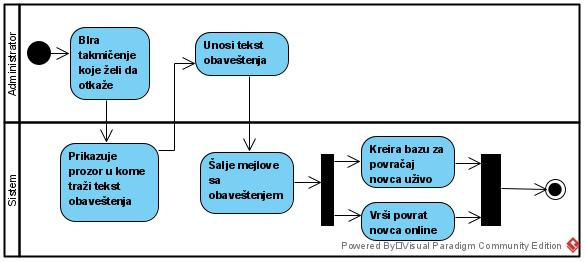
\includegraphics[scale=0.55]{sections/images/dijagram_aktivnosti_otkazivanje_takmicenja.jpg}
\end{center}
\caption{Dijagram aktivnosti za otkazivanje takmičenja}
\label{fig:kontekst}
\end{figure}

\end{document}